\chapter{Background and Related Work}\label{C:Background}

This chapter first describes the two layers that RPL runs on: the
\ieeemac{} layer and the \lowpanF{}
(\lowpan{}) adaptaion layer. It then introduces RPL and
explains how objective function can be used for load balancing.
Finally, it presents the simulation tools used in this work: the Contiki
operating system and the Cooja simulator, which emulates Contiki-based devices.
It also covers the basis of energy model used to estimate how much
the nodes consume.

\section{\ieeemac{}}
\ieeemac{} is a standard that defines the physical layer
(PHY) and media access control (MAC) for Low Rate
Wireless Personal Area Networks (LR-WPANs),
targeting devices constrained by low computing
power, memory and energy \cite{salmanOverviewIEEE8021542010}. It is
designed to operate in Personal
Operating Space (POS) of 10 meters or less and supports
three types of topology: star, peer-to-peer and mesh (a network that
connects a large number of nodes through relaying messages). The
standard offers three free bands
throughout the world with the throughput of 250\,kbps in the 2.4\,GHz
band 40\,kbps at 915\,MHz and 20\,kbps at 868\,MHz.

The 802.15.4 standard controls channel access with Carrier-Sense
Multiple Access with
Collision Avoidance (CSMA/CA). It defines two mode:
beacon-enabled for synchronous access and non-beacon-enabled for
asynchronous access.

In non-beaconed-enabled mode, nodes use unslotted
CSMA/CA, and they do not exchange request-to-send (RTS) and clear-to-send (CTS)
messages. When a node has packets to send, it delays the transmission for a
random backoff period. Afterward, it senses the medium and transmit
only if the channel is idle. If the channel is busy, the node waits for
another random backoff period and check the channel again.
Because transmissions are not synchronised, packets can arrive at any
time. As a result, nodes that may receive data have to keep their
radio on at all time.
This is especially costly in multihop topologies where nodes must
relay messages for other nodes.

In beacon-enabled mode, the coordinator cuts time into superframes,
which consists of 16 equally sized slots. Each
superframe starts when the coordinator sends a beacon to synchronise
the nodes. Each superframe has an active period and an optional
inactive period. During the active period, nodes compete for the
channel using slotted CSMA/CA, with backoff period aligned to the
slot boundary. During the inactive period, nodes can turn off their
radios until the next beacon to save energy.

\section{\ieeemacE{} Time-Slotted Channel Hopping}
The IEEE 802.15.4e amendment introduced Time-Slotted Channel Hopping
(TSCH), a MAC behavior that provides high reliability and time
critical assurances \cite{tsch}. TSCH achieves this by
combining time-division multiple access (TDMA) with frequency hopping.
Time is divided into fixed-length timeslots, and a group of
consecutive timeslots forms a \emph{slotframe}, which repeats
periodically. Nodes also switch channels from one timeslot to the
next according to a hopping sequence, as illustrated in
Figure~\ref{fig:tsch}. Spreading transmissions across channels in
this way reduces the effect of interference and multipath fading on
any single channel.

\begin{figure}
    \begin{center}
        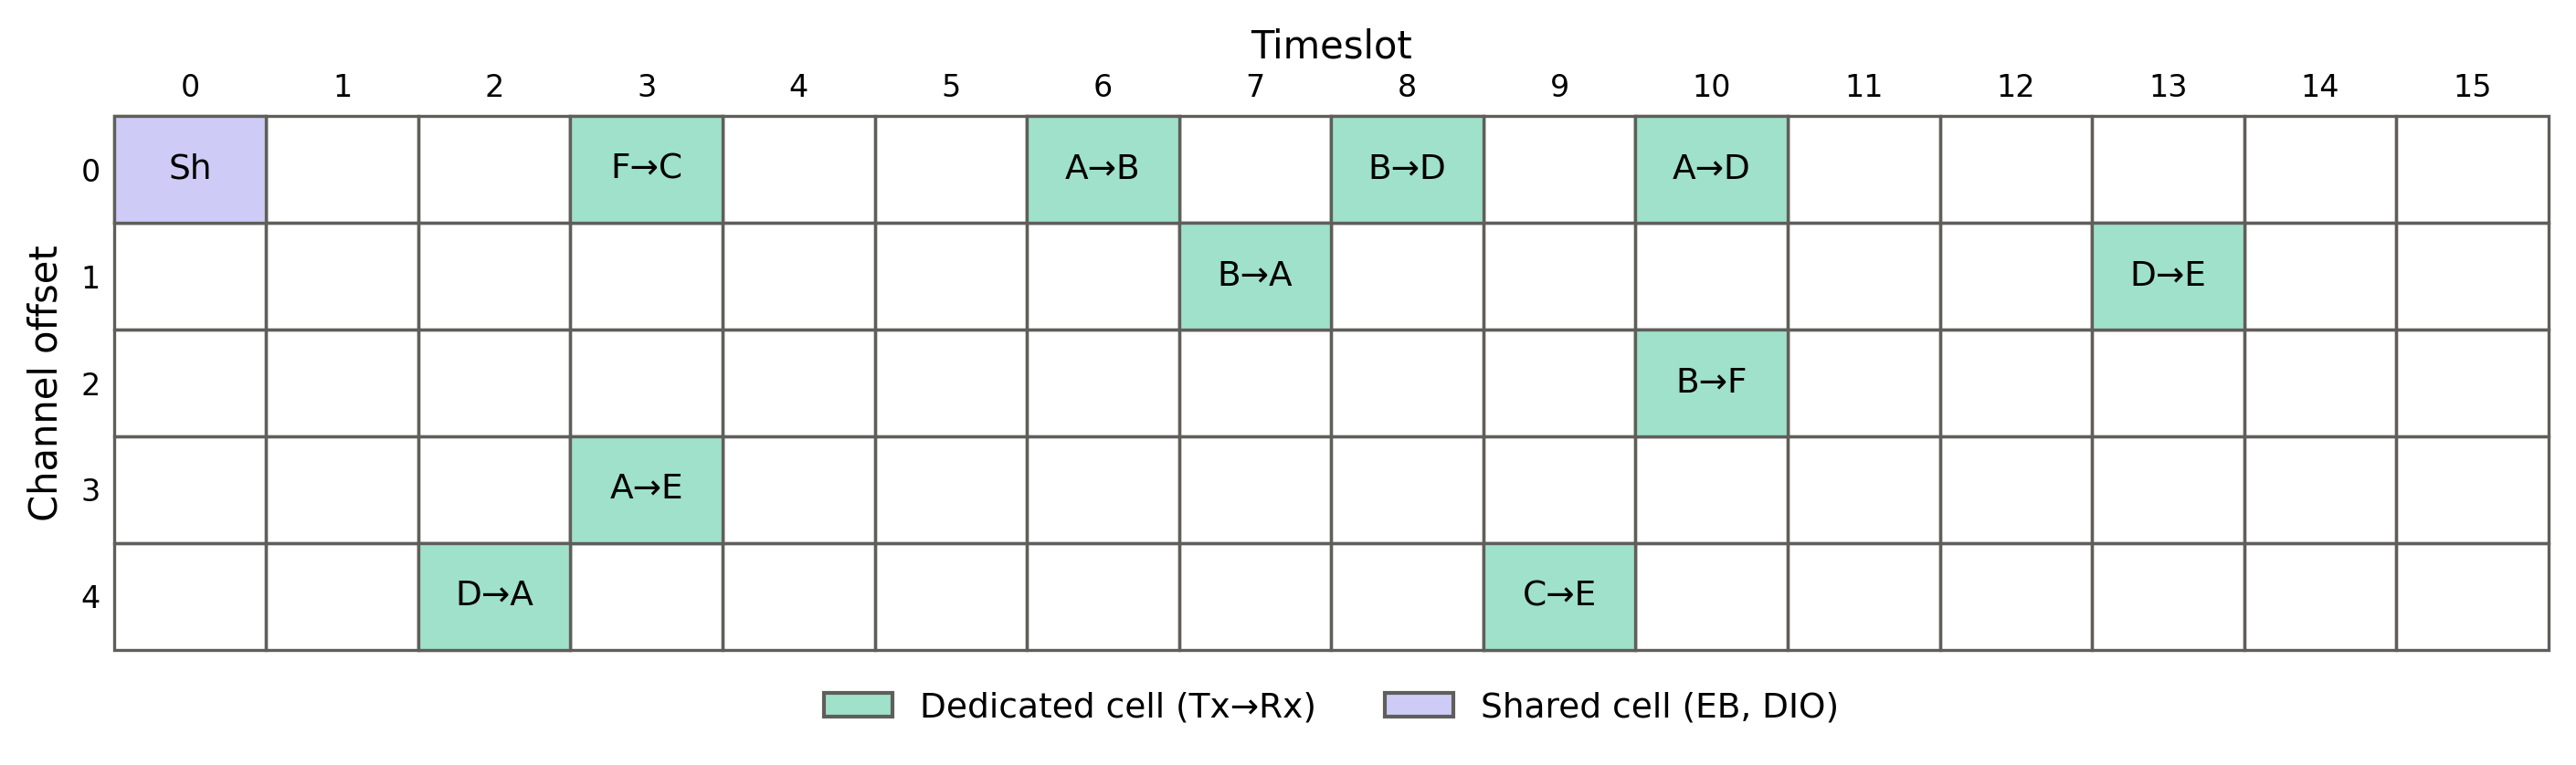
\includegraphics[width=0.9\textwidth]{assets/TSCH.png}
    \end{center}
    \caption{TSCH time slot visualisation.}\label{fig:tsch}
\end{figure}

A timeslot must be long enough that transmission and acknowledging
can be done within the duration of a slot. In each
timeslot, a node either transmits, receives or sleeps. A node with a
frame to send waits for a timeslot in which it is scheduled to
transmit, and then starts sending at a fixed offset from the start of
the slot. A node scheduled to receive turns on its radio shortly
before the expected start of the frame. If the node senses that it
does not have any data to receive after a short guard time, it turns its
radio off again for the rest of
the slot to save energy.

TSCH also uses channel hopping, so successive transmissions over the
same link use different frequencies. Each link is assigned a
channel offset, which lets different nodes communicate at the same time on
different channels. The frequency $f$ used for a transmission in that
link is
\begin{equation}
    f = F\left[(\mathit{ASN} + \mathit{channel\ Offset}) \bmod
    n_{\mathit{channel}}\right],
\end{equation}
where $n_{\mathit{channle}}$ is the number of available channels (16 in
the 2.4\,GHz band), Absolute Slot Number (ASN) is the total number of
timeslots that have elapsed since the network started
and $F$ is a lookup table that maps an index to a
physical channel.

TSCH avoids collisions through its schedule. Each transmission
occupies a \emph{cell}, identified by a slot offset within the
slotframe and a channel offset. In a \emph{dedicated} cell, only one
transmitter is scheduled, so the transmission is free of collision.
In a \emph{shared} cell, several nodes may transmit, and collisions
are handled by a CSMA/CA-like backoff. However, \ieeemacE{} does
not specify how the schedule is built or maintained, and leaves this
task to higher layers. One example is the approach of the IETF 6TiSCH
working group, which defines the 6TiSCH Operation Sublayer (6top)
\cite{rfc8480}, which lets neighboring nodes add and remove cells,
and the Minimal Scheduling Function (MSF) \cite{rfc9033}, which
decides when to do so.

Compared with CSMA/CA, TSCH offers higher reliability and lower
energy consumption. Reliability comes from two mechanisms: channel
hopping to reduce the impact of interference and multipath fading on
any single channel, and dedicated cells to allow nodes to transmit
simultaneously while avoiding collisions. The lower
energy consumption comes from nodes turning on their radio only in the
timeslots in which they are scheduled, and keep the radio off for the rest
of the slotframe.

These benefits come at a cost. TSCH is more complex than CSMA/CA: it
requires network-wide time synchronisation, which nodes must maintain
by periodically exchanging packets with their time source, and it
requires a schedule to be built and maintained. TSCH also introduces
latency, because a node with a packet to send must wait for its next
scheduled cell. The length of the slotframe therefore sets a
trade-off: a short slotframe gives nodes more frequent transmission
opportunities and lower delay, but forces them to wake up more often
and consume more energy

\section{IPv6 over Low-Power Wireless Personal Area Networks (6LoWPAN)}
Before 6LoWPAN, low-power wireless networks relied on proprietary or
non-IP protocol stacks such as ZigBee, since IP was considered too
demanding in computation and memory for constrained devices
\cite{culler20096lowpan}. Connecting these networks to the Internet
required gateways that translated between their protocols and IP,
which added complexity and limited interoperability.

% TODO: direct sentence, 6LoWPAn introduce bridge between layers...
6LoWPAN (IPv6 over Low-Power Wireless Personal Area Networks) brings
IPv6 to these devices, specifically to networks built on the
\ieeemac{} PHY and MAC layers \cite{rfc4944}. Using IPv6 end to end
simplifies interconnection with other networks and removes the need
for protocol-translating gateways. It also allows existing,
well-developed IP tools to be used for commissioning, configuring,
managing and debugging these networks.

Running IPv6 directly over \ieeemac{} is impractical because the two
were designed under very different assumptions. IPv6 targets
high-bandwidth links with large frames, requiring a minimum Maximum
Transmission Unit (MTU) of
1280 bytes, whereas \ieeemac{} targets low-power devices, with frames
of at most 127 bytes and data rates of up to 250\,kbps. To bridge
this gap, 6LoWPAN introduces an adaptation layer between the IPv6
network layer and the \ieeemac{} MAC layer, which provides three main
functions:

\begin{itemize}
    \item \textbf{Header compression.} An uncompressed IPv6 header
        occupies 40 bytes, which is a large share of a 127-byte
        \ieeemac{} frame.
        Many of its fields are either constant or can be derived from
        other layers; for example, the source and destination addresses
        can often be reconstructed from the link-layer addresses. 6LoWPAN
        omits or shortens these fields to reduce header size.
    \item \textbf{Fragmentation and reassembly.} IPv6 requires every
        link to support a minimum MTU of 1280 bytes, whereas an
        \ieeemac{} frame carries at most 127 bytes. 6LoWPAN splits
        IPv6 datagrams that do not fit into a single frame into
        fragments and reassembles them at the receiver.
    \item \textbf{Link-layer forwarding.} 6LoWPAN optionally supports
        forwarding packets across multiple hops at the link layer
        (\emph{mesh-under}). Alternatively, routing can be performed at
        the IP layer (\emph{route-over}), which is the approach taken by
        RPL.
\end{itemize}

\section{Routing Protocol for Low-Power and Lossy Networks (RPL)}

RPL is an distance-oriented vector routing protocol that builds a
Destination-Oriented Directed Acyclic Graph (DODAG) over IEEE
802.15.4 PHY/MAC layers and 6LoWPAN \cite{alexanderRPLIPv6Routing2012}.
It is primarily designed for Wireless
Sensor Networks (WSNs),
where multipoint-to-point traffic toward one or more roots is the
predominant communication pattern.
Routes in RPL are optimised for traffic to or from one or more
roots in the topology, while maintaining reliable and energy
efficient data collection. To maintain reliable and energy-efficient
data collection, RPL is designed to adapt to changing
network conditions, allowing nodes to switch routes when route
degradation is detected.

\subsection{Destination-Oriented Directed Acyclic Graph (DODAG)}
RPL organises nodes under a DODAG, with the WSN's sink
node often serving as the root of DODAG. A node forwards packets
toward the root by relaying them to its
parent, which in turn relays them further up the tree until they reach the root.
In a multi-sink deployment,
each sink node serves as the root of its own separate DODAG.
Within a DODAG, each node maintains a rank value, which is an estimation of the
distance between itself and the DODAG
root. This value is used to determine a direct parent link, which
must have a lower rank,
creating a herarchy network toward the root as illustrated in
Figure~\ref{fig:dodag-example}. This means that the rank are
monotonic increasing and the root has the lowest rank in DODAG.

A node's rank is computed by an objective function (OF). The OF
converts one or more metrics into rank, and it also determines how a
node selects its preferred parent. The RPL
specification does not mandate a single OF for all applications.
Instead, RPL separates its core routing operationg, such as DODAG
construction and maintainance from from route optimisation, which is
delegated to the OF. RPL also allows having multiple DODAGs in the
samework, in which each
DODAG would have a different OF for different purposes. This lets
each deployment choose the OF that best fits its requirement, such as
minimising energy consumption, reducing latency, or improving link
quality.
As a result, RPL can support a wide range of LLN applications without
changing the protocol itself.

\begin{fig}[ht]
    \begin{center}
        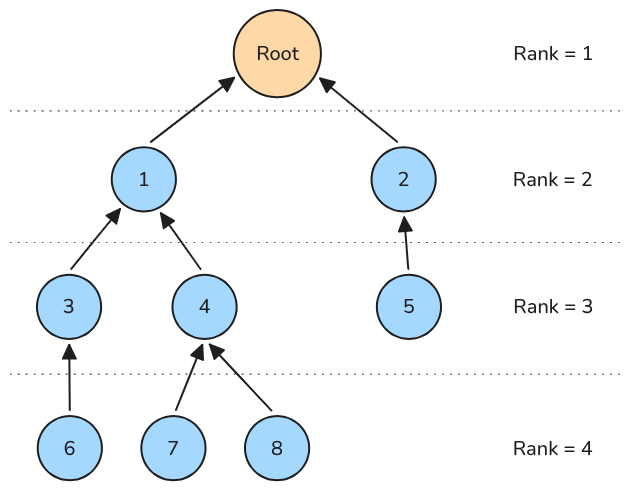
\includegraphics[width=0.6\textwidth]{assets/dodag.png}
        \caption{Example of a DODAG topology, showing nodes organised
        into a hierarchy rooted at the sink node.}
        \label{fig:dodag-example}
    \end{center}
\end{fig}

During DODAG construction, each node selects a parent from a pool of
candidate parents, which are neighbouring nodes that have already joined the
DODAG. For each candidate parent $P$, the note $N$ computes the rank
it would have if it chose $P$:
\begin{equation}
    \mathit{Rank}(N) = \mathit{Rank}(P) + \mathit{Rank\_Increase}
\end{equation}
where $\mathit{Rank}(N)$ is the resulting rank of the node $N$,
$\mathit{Rank}(P)$ is the rank advertised by the candidate parent $P$,
and $\mathit{Rank\_Increase}$ is a positive value computed by the OF
that represents the cost of using $P$ as a parent. Because
$\mathit{Rank\_Increase}$ is always positive, a node's rank strictly increases
with each hop away from the root. How $\mathit{Rank\_Increase}$ is computed
and how parent is selected depends on the OF in use,
as discussed later in this chapter.

RPL introduces four types of control messages to form
and control DODAG, as specified in ICMPv6 via RFC 6550
\cite{alexanderRPLIPv6Routing2012}
\begin{itemize}
    \item DODAG Information Object (DIO): a DODAG advertisement message,
        carrying information that
        allow nodes to discover a RPL instance, select parents and
        maintain the DODAG.
    \item DODAG Information Solicitation (DIS): a request message
        when a node wants to join a DODAG.
    \item Destination Advertisement Object (DAO): a node
        advertisement message, indicating that it has joined DODAG
        and is reachable for downward route.
    \item Destination Advertisement Object Acknowledgement (DAO-ACK):
        the acknowledgement of the root, confirming the downward path
        to the node.
\end{itemize}

To begin the DODAG forming process, the root node sends its DIO to
its neighbouring nodes, carrying RPL indentifiers and any
additional metrics required by the OF. Upon receiving DIO, a node
compares its rank with the advertised rank and filters out ranks that
are higher then its own to prevent loop formation. Afterward, the node decides
whether to join the advertised DODAG or not.
In certain implementations, nodes wait for several DIOs, building
the pool of candidate parents before deciding.
After joining DODAG, the node computes the path cost of the
corresponding link for each candidate and determines the preferred
parent according the OF's policy.
Once a parent has been selected, the node broadcasts its own DIO to
advertise itself to its neighbours. This process is repated
outward through the network until every node has join the DODAG.
% TODO: may include diagram of how DIO transmission work

DIOs are crucial in maintaining DODAG. Nodes send DIOs periodically to
advertise their rank and routing metrics. Each time a node receives a
DIO, it update the candidate parent set and
recompute its rank through each candidate in the same way as when it
first joined the DODAG. If the node switches its
preferred parent or its rank changes, it sends a new DIO to spread
the update down the DODAG. This lets the DODAG adapt as link
conditions and traffic change.
Despite that, frequent DIO would be redudant in consistent network
conditions, thus RPL employs Trickle timer to regulate the emission
of DIO based on network consistency.

A node does not need to wait passively for a periodic DIO to join a DODAG.
It can request DODAG information by broadcast a DIS message. The
response depends on how the
DIS is sent. If a neighbour receives a unicast DIS, it must reply with a
unicast DIO and must not reset its Trickle timer. If a neighbour
receives a multicast DIS, it resets its Trickle timer, so the node soon
receives DIOs from all nearby DODAG members. When the node receives a
DIO sent in response to its DIS, it processes the DIO in the same way
as a periodic DIO.

When a node joins DODAG, it also sends a DAO to advertise that it can be
reached downwardly. The DAO's destination depends on the Mode of
Operation (MOP). In storing mode, the node sends the DAO to its
preferred parent, and
each parent stores the route and forwards the information further up
the DODAG. In non-storing mode, the node sends the DAO directly to the
root. The root then keeps the full set of downward routes and uses
source routing to reach each node. A node can ask for an
acknowledgement by setting a flag in its DAO. The receiver, which is
the parent in storing mode or the root in non-storing mode, then
replies with a DAO-ACK. If the node receives no DAO-ACK, it retransmits
the DAO.

% TODO: downward route?
The downward are supported to P2MP and P2P route, in which the
destination is not the root node. In this pattern, the node sends DAO
to its preferred parent in a unicast manner

% TODO: study the storing mode more
In this pattern, the RPL specification defines two mode: storing mode
and non-storing mode. In storing mode, the downward routing tables
are included in each nodes
However, in non-storing mode, the downward routing tables are stored
only in the DODAG root. This means that P2P communication need to be
forwarded to the root node, where the root would then formulate the
routing path to the downward node.

% TODO: clarify this
The specification also opens option to specify DAO-ACK or not. A node
would only consider reachable only after it has received the DAO-ACK.

% TODO: include how DODAG maintain loop free
\subsection{DODAG Maintainance}
Local repair
Poisonining

% TODO: write more about trickle timer
\subsection{Trickle Timer}
Trickle timer is a scheduling algorithm based on consistency model.
The algorithm is structured in a way that would promptly send out DIO
during the formation process and would slow down when the DODAG has
been stablised to reduce redundant DIO transmission \cite{rfc6206}.

The Trickle timer does this by evaluating the consistency of the
network message with its own state.
When the network information is consistent, it
exponentially increases the transmission interval of DIO. However,
upon detecting inconsistencies, trickle timer reset its send interval
to boost DIO transmission to spread the latest information to the
rest of the DODAG.
However, the RPL standard does not fully define what counts as an
inconsistency. It lists a minimum set of events that must restart the
Trickle timer: joining a new DODAG version, receiving a multicast
DIS; and detecting a routing loop or another inconsistency while
forwarding a packet. The specification states that this list is not
exhaustive and that implementations may treat other events as
inconsistencies. Contiki-NG, for example, also resets Trickle timer
when a node's rank change by more than a threshold.

% TODO: I_max, specify that this is the doubling interval
Trickle Timer employs three configuration
parameters to determine the sending window of DIO: $I_{\mathrm{min}}$,
$I_{\mathrm{max}}$ and $k$ as shown in Table~\ref{tab:tricker_timer_params}.
The maximum sending interval time
$I_{\mathrm{max\_time}}$ is calculated as:
\begin{equation}
    I_{\mathrm{max\_time}} = I_{\mathrm{min}} \times 2^{I_{\mathrm{max}}}
\end{equation}

The Trickle algorithm controls the transmission interval $I$, which
always stays within $[I_{\mathrm{min}}, I_{\mathrm{max}}]$. In RPL,
the initial interval is usually $I = I_{\mathrm{min}}$.
At the start of each interval, Trickle sets a counter $c$ to $0$. It
then picks a
transmission time $t$ uniformly at random from $[I/2, I)$. During the
interval, $c$ increases by one each time the node hears a consistent
message from a neighbour. At time $t$, the node transmits only if
$c < k$, where $k$ is the redundancy constant. Otherwise, it suppresses
the transmission. When the interval ends, Trickle doubles its length,
up to the maximum:
\begin{equation}
    I = \min(2I,\ I_{\mathrm{max}})
\end{equation}
If the node detects an inconsistency while $I > I_{\mathrm{min}}$, it
resets $I$ to $I_{\mathrm{min}}$ and starts a new interval.

\begin{table}
    \caption{Trickle Timer Parameters}\label{tab:tricker_timer_params}
    \begin{center}
        \begin{tabular}[c]{@{}p{0.22\linewidth}p{0.10\linewidth}p{0.58\linewidth}@{}}
            \hline
            \textbf{Parameter} & \textbf{Symbol} & \textbf{Description} \\
            \hline
            Min interval length & $I_{\mathrm{min}}$ & The minimum sending
            interval between two messages \\ % TODO: problably fix this
            Max interval length & $I_{\mathrm{max}}$  & The maximum number of
            times that the sending interval can double \\
            DIO redundancy constant & $k$ & The number of consistent
            DIOs before suppresses its own DIO transmission \\
            \hline
        \end{tabular}
    \end{center}
\end{table}

\subsection{OF0 and MRHOF}

Up to now, the IETF ROLL working group has standardised only two
objective functions: Objective Function Zero (OF0) \cite{rfc6552} and
Minimum Rank with Hysteresis Objective Function (MRHOF) \cite{rfc6719}.

% TODO: talk more about step of rank
OF0 was developed to be a simple objective function that utilises step
of rank, which is an intermediate computation based on link
properties of a certain neighbour, and computes $\mathit{Rank\_Increase}$ as
\begin{equation}
    \mathit{Rank\_Increase} = (\mathit{Rf} \times \mathit{Sp} +
    \mathit{Sr}) \times \mathit{MinHopRankIncrease}
\end{equation}
where $\mathit{Rf}$ (Rank Factor) is a small positive integer used to scale
the step of rank; $\mathit{Sp}$ (Step of Rank) is an integer value
representing hop count in
abstract sense; and $\mathit{Sr}$ (Stretch of Rank) is used to inflate
$\mathit{Rank\_Increase}$ for
hysteresis, preventing the OF from switching parents constantly.
We can select OF0 parameters by selecting $\mathit{Rf} = 1$,
$\mathit{Sp} = 1$ and $\mathit{Sr} = 0$,
which reduces $\mathit{Rank\_Increase}$ to a simple fixed per-hop
increment of 256. However, the specification of OF0 strongly
recommends computing step of rank
from Expected Transmission Count (ETX) to avoid blind hop count
measure, where it would select furthest
node whose link might be noisy and lossy to reduce the number of hops.
% TODO: Include Convert ETX to step of rank

OF0 can be regarded as implicitly using hop count as
routing metric. This mean that the traffic from OF0 follow the shortest path
to root without considering any load balancing requirement.
However, this also means that OF0 does not consider other link
qualities such as latency, energy residual in its calculation as well
as might choose worse off route but have the shortest hop count to root.
This led to the introduction a more sophisticated MRHOF.

In contrast, MRHOF propose multiple thresholds call hysteresis for
path cost and time
. In path cost threshold, unless the
potential node is better than the current parent by a threshold, it
will stick with the current parent. However, after the time
threshold, if that node is still better then the node will switch
parent. This would allows a more stabilised DODAG. Additionally,
MHROF allow choosing one from various metrics as the determing factor.

The default metric of MRHOF is Expected Transmission Count (ETX)
metric. The main goal of ETX is to select routes with high end-to-end
through put:
\begin{equation}
    \mathit{ETX} = \frac{1}{D_t \times D_a}
\end{equation}
where $D_t$ is the probability that the receiving node receives the
packet and $D_a$ is the probability that the transmitting node
receives acknowledgement packet is successful. So ETX is the average
number of packets need to send and acknowledgement.
Since ETX is a floating point number while devices RPL operates on do
not generally support floating point arithmeic. The specifcation
indicates that 128 would be 1.0 ETX, improving the performace with
bitshift instead of expensive division.

% TODO: what word to describe route need less packets TX
In essense, using ETX as metrics focus on more transmission-efficient route.

There are two thresholds in MRHOF, rank threshold and time threshold.
The specification define $PARENT\_SWITCH\_THRESHOLD$ as the minimum
path cost improvement before deciding to switch.
There is time threshold, meaning that if a node consistently perform
better but not more than the ETX threshold, it still switch.

% TODO: include other metric container
The specification also open the choices of the routing metrics to energy,...
However, ETX is the more popular choice when it comes to MHROF.

Thanks to the flexibility of DIO header option.
% TODO: talk about the flexiblity of DIO

\section{Load Balancing in RPL}
Load balancing is an important issue in WSNs since devices are
expected to operate on battery for a long period of time. Some nodes
are used more frequently than others, especially the nodes near the
root, and exhaust their energy rapidly. These also includes when
there is an imbalance the traffic rate between node, where certain
nodes have higher data traffic than others e.g. videos or images,
thus selecting one parent would exhaust the possible routes to the parent node.

In this sense, load balancing is about distributing load from the
leaf to root node so that the node within the same hop share the
loads more evenly

These have to account for bursty traffic

% TODO: define what is load balancing
Despite that, RPL does not consider load balancing since it is
oriented to handling
low data traffic. Therefore, the network suffers in terms of latency,
delivery ratio and energy consumption under imbalance load senerios.

This is where OF0 and MRHOF fall short as they only consider one
metric: hop count and ETX. This does not capture the different
load of each node. Generally, ETX value does not change much when a
node experience heavy load \cite{kimQURPLQueueUtilization2015}

Another problem in load balancing is Thundering Herd problem, when a
new node join the DODAG and advertise its existence. Since this node
does not have any load, the neighbouring nodes would then choose this
as their prefered parents, potentially overloading this node. While
leaving their current parent free of load. When the current parent
advertise itself, all the node would then switch, thus creating
switch back and forth.
% TODO: insert image for thundering herd

% TODO: include other problems in load balancing as well

\section{Review of RPL Objective Functions Load Balancing}
Various objective functions have been proposed, which can be
categorised into 4 groups: single metric, composite and context aware.

OF0 and MRHOF fit into single metric category.

% TODO: maybe include more OF0 and MRHOF evaluation
\cite{pradeskaPerformanceAnalysisObjective2016} evaluate  the
performance of OF0 and MRHOF in COOJA Contiki
Additionally, ... evaluates the performance of the standardised OFs
and find performance of OF0 degrade upon increasing load

In \cite{kimQURPLQueueUtilization2015}, the authors argues that most
of the packet losses are due to queue loss. Thus they proposed QU-RPL
--- an objective function that uses queue utilisation metric
--- to avoid queue overflow from parents with little free queue.
In addition to  a new routing metric, they also
modified the trickle timer to reset when a node experiences
consecutive queue losses for timely repair when links degrade. With
the changes, they achive lower queue
loss ratio and a more balance tree.
% TODO: wording
However, only queue metrics are
taken into consideration without taking hop count or ETX into
account, thus choosing parents that are free but lead to losses in
delivery ratio.

A new objective function OF-FL is presented in
\cite{gaddourOFFLQoSawareFuzzy2014}, which employs fuzzy logic with
four metrics with the aim of supporting various application requirements.
The authors used four metrics hop count, end to end delay, battery
level and ETX to categorise link quality. Each metric follows fuzzy
logic and indicate link quality from awful to excellent. The
simulation results show that OF-FL achieve higher PDR while
conserving more energy. Despite that, the process of encoding each metrics
into quality label is done manually and subject to the biases of the
doers. % TODO: more about limitation in this

The authors presents Energy-Aware Objective Function (EAOF) for
healthcare monitor application in
\cite{abreuEnergyawareRoutingBiomedical2014}. Biomedical sensor nodes
are small and operate on battery-powered. Traditional routing methods
tend to choose most reliable route, meaning that a small number of
routes are selected, thus deplete enegy faster. In this paper, they
avoid such problem and achieve a more balance energy usage through
utilising ETX and remaining energy, indicating how much battery power
each potential forwarding node has left. EAOF trades a small
reduction in packet reception for better energy balance and longer
network lifetime.
% TODO: what is the limitation

% TODO: finish the below
The authors in \cite{taghizadehCLRPLContextAwareLoad2018} proposed
Context-Aware and Load Balancing RPL (CLRPL). They introduced a new
metric called Context-Aware Routing Metric (CARM), which considers
queue utilisation and the percentage remaining power of a entire
parents' chain from root the the node instead of the immediate
parent. CARM would cnosider low-power parent but high-power overall
route instead of rejecting it like energy of a single parent.
% TODO: include limitation of this

\cite{liuLoadBalancedRouting2013} introduces LB-RPL. While still
considering communication quality, LB-RPL add two mechanisms:
A node would keep the table of top k parents and have proability of
forwading a packet i to node j through the equation.
And node with higher buffer utilisation delay their DIO message,
avoiding neighouring nodes select it as the parent. In the
simulations, they achieve better PDR, reduce latency and
substaintially reduce the workload of nodes near the root. Despite
that, forwading a packet to two parents duplicate the traffic while
only achieve same throughput.
calculate the load differences between parents to make parent switch
decision. % TODO: more on this

\cite{homaeiLoadBalancingIoT2025} uses learning automaton (LA) inear
Reward-Penalty (L\_R-P) updating scheme. Utilising traffic index, hop
count to root and remaining energy level. Reward the parent for
successful transmission. Also update the Trickle Timer to increase
DIO transmission when traffic is low.
% TODO: talk about this

Weighted Random Forward RPL (WRF-RPL) was propsoed in
\cite{acevedoWRFRPLWeightedRandom2021}, which would select parents
randomly based on weighted score % TODO: more about this
They would set $Rank\_Increase$ to fixed 1 thus making the rank hop
count to root. They use node's remaining energy for the parent's
weight calculation. Nodes with higher weights are more likely to be
selected to forward packets, however, nodes with low weights can
still be selected, albeit with lower chance. This spreads traffic,
reduce congestion and avoids repeatedly using a single relay node.
The author note that the performance of the OF depends on the
topology, network with more imtermediate nodes are able to spread the
load more evenly compared to leaf-dominant network.

In recent, there has been many attempts to employ machine learning
into OFs. Despite that, most of the new application of ML in RPL
focues on reinforcement learning
with little focus on supervised learning

In \cite{duenassantosQRPLQLearningBasedRouting2024}, the authorse
puts Q-Learning to OF, award the model when a packet is trasmitted
successfully and penalise when choosing a link that lead to packet
loss. The model learns from real packet outcomes rather than from a
pre-trained model. The reward scheme is based on the number of
transmission to the next hop. Nodes start by selecting parent at
random and then gradually shifts to best-known parent. Additionally,
each node also advertises its Q-value in DIO to neighouring nodes.
In addition to that, the authors also use ETX and RSSI to break ties
between parents and filter unsuitable nodes.
The model performance settles after roughtly 2-3 hours.
Yet, the paper did not include memory or model overhead analysis or
the cost of exploration when the model first starts learning.

\cite{faragCongestionAwareRoutingDynamic2021} buils upon
\cite{kimQURPLQueueUtilization2015} by incorperating reinforcement learning
, similar to ... argues that most of the losses are from queue loss.
Using reinforcement learning to select parent with less full queue
Additionaly, the author employs softmax parent selection strategy,
which choose parents based on weights to avoid Thundering Herd Problem.
The evaluation is done in Monte Carlo simulations in MATLAB instead
of standard network simulator.
Not really Q-learning, the update does not have discount factor. And
tested on very heavy traffic 30-120 packets per minute per node.

\cite{sangeethaFederatedLearningBasedParent2025} employs federated
learning to train the weights on fly and update the optimal weight
through DIO messages.
The model predicts the energy cost of routing through each candidate
parent and picks the lowest.
They use deep learning MLP as the model.
The model takes in four inputs ETX, hop count, residual energy and delay)
Report they have better energy consumption and network lifetime than
OF0 and MHROF.
Each node learn from the data and send the weights to the root node.
The root node then compile and put all of them together before
forwading it to each nodes in the network.
The energy is measured by measureing the Python running time and map
it to Sky mote energy usage.
However, the objective function wasted using Cooja mote in Cooja
simulator, which is compile and run on host machine without
constrained on device computational power or memory. They claim of
using ContikiMAC duty cycling with Contiki-NG without mentioning they
port the mode, which contradict our finding about Contiki-NG.

However, we found out that there are little researches on applying
supervised machine learning model in RPL. To our best knowledge,
there are three papers about
We found a research group
that proposed using machine learning techniques to predict the chance
of packet forwarding successfully on each hop.

In RPL+, the authors
used Decision Tree to perform feature importance evaluation with
six metrics ETX, channel utilisation, density, through put, queue
utilisation and MAC losses on data gathered hop by hop from
simulation \cite{duenassantosRPLImprovedParent2022}. They set
the $\mathit{Rank\_Increase}$ fixed to 1, which can be regarded as hop count,
and use the feature
importance as coefficients in linear equation and select parent with
the lowest score. Even though they improve the performance of PDR and
delay, the random forest model is only for feature importance
analysis and the training data only consider the success chance of
forwarded by one hop instead of the whole path. Additionally, having
fixed $\mathit{Rank\_Increase}$ means that the OF would select
parents with the shortest hop count.

In \cite{mezherGNBRPLGaussianNaive2023}, the research group train a
Naive Bayes classifier to predict the probability of a packet is sent
successfully or not on the same training feature as RPL+. This assume
that the distribution of the features fall into Gaussian distribution
In this paper, they train on more data and integrate the model into
the OF. However the evaluation lacks consideration for OF0.

Subsequently, the group proposed ML-RPL, using CatBoost model to
learn from eight metrics namely hop count, ETX, MAC losses, density,
channel utilisation, throughput, queu utilisation and RSSI
\cite{santosMLRPLMachineLearningBased2023}. Similar to previous
researches, this model predicts the predict the probability of
successfull one hop transmission. The evaluation of the results lack
energy or cpu util evaluation, and lack evaluation of the model size
given the context of constrained devices.

\section{Contiki Operating System and COOJA Simulator}
\subsection{ContikiOS and Contiki-NG}
Contiki is a lightweight operating system (OS) built for constrained
devices in WSN with a few kilobytes of RAM and tens of kilobytes of
flash memory to run \cite{contiki}.
Originally developed by Adam Dunkels in 2002, it has since received support
from a community of developers, industrial partners and research institutions.
Contiki has been ported to a wide range of architectures, from 8-bit
AVR processors to
16-bit TI MSP430 and 32-bit ARM Cortex-M devices.
The MSP430 family is the most widely used target in WSN research
because of its very low power consumption, and it is the basis of several
popular sensor motes that the Cooja simulator can emulate at the instruction
level.

At its core, Contiki uses an event-driven kernel, where all processes
run on a single shared stack, to save memory compared to
multi-threaded systems where each thread has its own stack. The drawback is that
event-driven code is hard to write: any task that waits for an event,
such as a timer or an incoming packet, has to be split across several
callbacks and coordinated through an explicit state machine. Contiki
addresses this with \emph{protothreads}, lightweight stackless threads
that provide a conditional blocking wait \cite{dunkels2006protothreads}.
A protothread can wait for an event in the middle of a function and
resume from the same point when the event occurs, so the code can be
written as a linear sequence of steps, removing most
explicit state machines while adding only about two bytes of memory
per thread. % TODO: need to understand this

Contiki also ships with a full network stack for WSNs. Its uIP stack
supports both IPv4 and IPv6, and IPv6 runs over \ieeemac{} through the
6LoWPAN adaptation layer, with RPL as the routing protocol. Contiki
further adds a radio duty cycling (RDC) layer between the MAC layer
and the radio driver, and provides several low-power RDC protocols,
such as X-MAC, LPP and ContikiMAC, which were developed before TSCH
became standardised. Of these, ContikiMAC became the default.

In November 2017, Contiki-NG (Contiki Next Generation) was released
as version 4.0, a fork of the original Contiki under the 3-clause BSD
license \cite{ContikiNG}. It targets modern IoT devices,
mainly 32-bit MCUs such as ARM Cortex-M3, and focuses on reliable and
secure standardised protocols like IPv6/6LoWPAN, 6TiSCH, RPL, and CoAP.
To this end, Contiki-NG removes the support for 8-bits and 16-bits
platforms, and older, experimental and non-standarised protocols. It
drops the non-IP Rim and IPv4 support, making the system IPv6-only.
It also removes the RDC layer, leaving only CSMA, \ieeemacE{} TSCH
and a minimal \texttt{nullmac}, a MAC layer that neither sends or
receives packets.
Although the main support of Contiki-NG is 32 bits MCUs, several older 16-bit
MSP430 platforms such as Tmote Sky and Zolertia Z1 are still
maintained, and can be emulated in Cooja simulator.

Contiki-NG also rewrote the RPL implementation called RPL-lite and
make the new version default RPL implementation in the system.
The original Contiki implementation is still kept and is called RPL-classic.
Draws from years of experience, RPL-lite drops several RPL features
that are rarely needed in practice.
It only supports a single RPL instance with only one DODAG at a time, and
only the non-storing mode of operation, in which the root node holds
all the downward routes.
For MRHOF, RPL-Lite adds a time-based hysteresis on top of the
standard rank hysteresis, so that a node eventually switches to a
parent that has been consistently better for a long period, even if
the difference stays below the switching threshold.

\subsection{Cooja Simulator}
Cooja is a network simulator tool distributed with Contiki-NG. It is
capable of emulating hardware motes to instruction level from
firmware image built for a real platform
or software motes, which run Contiki compiled for the host machine.
Out of the box, Cooja provides two hardware mote types: Tmote Sky
(TelosB) and Zolertia Z1 with the platform specifications shown in
Table~\ref{tab:mote-specs}, and a software-based mote type called Cooja.

For hardware emulation, Cooja uses \texttt{MSPSim}, a Java-based
instruction-level emulator, to emulate the MSP430 family MCUs with
cycle accurate, including timing, memory limits and peripherals.
The Cooja mote, in contrast, is not time-accurate and is compiled to
run directly on the host
machine and bypass the limitations of computation power or memory on
real hardware. This makes the simulation using Cooja motes much
faster but less accurate in terms of time, energy and computational
resource usage. For this reason, Cooja mote is typically used to test
the protocols and
application logic quickly before running the slower but more accurate
hardware emulation.

\begin{table}[h]
    \caption{Supported mote hardware specifications in COOJA simulator}
    \label{tab:mote-specs}
    \begin{center}
        \begin{tabular}{lll}
            \hline
            \textbf{Specification} & \textbf{Zolertia Z1} &
            \textbf{TMote Sky} \\
            \hline
            Microcontroller        & MSP430F2617      & MSP430F1611 \\
            CPU                    & 16-bit RISC @ 16\,MHz     &
            16-bit RISC @ 8\,MHz \\
            RAM                    & 8\,KB                     & 10\,KB \\
            Flash memory           & 92\,KB                    & 48\,KB \\
            Transceiver            & CC2420, IEEE 802.15.4     & CC2420,
            IEEE 802.15.4 \\
            Frequency band         & 2.4\,GHz                  & 2.4\,GHz \\
            Data rate              & 250\,kbps                 & 250\,kbps \\
            \hline
        \end{tabular}
    \end{center}
\end{table}

\section{Energy modeling}
Contiki-NG estimates energy consumption using a
software-based online mechanism proposed in
\cite{dunkelsSoftwarebasedOnlineEnergy2007}. It uses a linear
model in which each hardware component such as the CPU, the radio transmitter
and the radio receiver, draws a roughly constant current while it is active.

The total energy is then the sum of each component's active time
multiplied by its average current draw and the supply voltage:
\begin{equation}
    E = V \sum_{i} I_i \, t_i ,
\end{equation}
where $V$ is the supply voltage, $I_i$ is the average current draw of
component $i$, and $t_i$ is the time it spent active. Because the
estimation runs entirely in software, it needs no additional
measurement hardware and can easily be ported to different platforms.

Contiki-NG implements this model in its \emph{Energest} module, which
records how long each
component stays in each power state, measured in timer ticks.
Energest tracks give states. Three describe the MCU: active (CPU),
low power mode (LPM),
deep low power mode (DLPM). The other two describe the radio:
transmitting (TX) and receiving (RX). So the energy estimate in
Contiki-NG is calculated as follow. The time $t_x$ spent in each state is
obtained by dividing its tick count by the number of ticks per second
\begin{equation}
    t_x = \mathit{ticks}_x / \mathit{ENERGEST\_SECOND}
\end{equation}
And the energy consumed by a node is estimated as
\begin{equation}
    E = V \left( I_{\mathrm{CPU}}\, t_{\mathrm{CPU}}
        + I_{\mathrm{LPM}}\, t_{\mathrm{LPM}}
        + I_{\mathrm{DLPM}}\, t_{\mathrm{DLPM}}
        + I_{\mathrm{TX}}\, t_{\mathrm{TX}}
    + I_{\mathrm{RX}}\, t_{\mathrm{RX}} \right),
\end{equation}
where $V$ is the supply voltage, and $I_x$ and $t_x$ are the
average current
draw and the time spent in each state. In many cases where the energy
estimation is used to compare between
homogeneous nodes within the same network, V does not need to be
explicitly calculated to simplify the calculation.

The value of current drawn of each state is gathered from the
datasheet of the MCU and transceiver. Table~\ref{tab:current-draw}
shows the current drawn
of two platforms Z1 \cite{zolertia_z1} and Tmote Sky
\cite{moteiv_tmotesky} with transceiver CC2420 \cite{ti_cc2420}. However, the
current draw from datasheet is only taken as a reference
point as it can vary a lot in different situation.

% TODO: what should I do with Z1 CPU active at 8mhz
\begin{table}[ht]
    \centering
    \caption{Average current draw per Energest state for the Zolertia
    Z1 and Tmote Sky platforms.}
    \label{tab:current-draw}
    \begin{tabular}{llcc}
        \hline
        \textbf{Component} & \textbf{State} & \textbf{Z1} &
        \textbf{Tmote Sky} \\
        \hline
        MCU   & Active (CPU)                 & 10\,mA       & 1.8\,mA \\
        & Low-power mode (LPM)         & 23\,$\mu$A   & 54\,$\mu$A   \\
        & Deep low-power mode (DLPM)   & 0\,$\mu$A    & 0\,$\mu$A    \\
        \hline
        Radio & Receive (RX)                 & 18.8\,mA     & 18.8\,mA     \\
        & Transmit (TX)                & 17.4\,mA     & 17.4\,mA     \\
        \hline
    \end{tabular}
\end{table}

% TODO: wording
In CSMA mode, the radio is turn on at all time, thus the difference
in energy usage between nodes using this energy model is mainly
difference in CPU utilisation and pretty negligible as CPU energy
consumption is much smaller than that of radio. In contrast, TSCH and
radio cycling allow nodes to turn off their radio if their is no
packet intended for them, the energy consumption would be much bigger
for nodes that have high traffic.

\section{Hardware Selection}
% TODO: do this
However, TSCH is a much more complicated and memory heavy algorithm
for such old devices Sky and Z1. Hence we opt for CSMA and use active CPU ticks
as intermediate value to measure the energy consumption relative to
other nodes in the network.

\begin{table}[htbp]
    \centering
    \caption{Memory footprint of the Contiki-NG \texttt{rpl-udp}
        example with \texttt{QUEUEBUF\_CONF\_NUM}=8 and
        \texttt{NBR\_TABLE\_CONF\_MAX\_NEIGHBORS}=10.
        Z1: 92\,KB flash, 8\,KB RAM; Tmote Sky: 48\,KB flash, 10\,KB RAM.
    All values in bytes.}
    \label{tab:footprint-nbr10}
    \begin{tabular}{lllrrrrr}
        \hline
        Platform & MAC & Node & \texttt{.text} & \texttt{.data}
        & \texttt{.bss} & Flash & RAM \\
        \hline
        Z1  & CSMA & udp-client & 43\,788 & 350 & 6\,002 & 44\,138 & 6\,352 \\
        &      & udp-server & 43\,412 & 350 & 5\,946 & 43\,762 & 6\,296 \\
        \cline{2-8}
        & TSCH & udp-client & 56\,092 & 398 & 7\,962 & 56\,490
        & 8\,360$^{\dagger}$ \\
        &      & udp-server & 55\,716 & 398 & 7\,906 & 56\,114
        & 8\,304$^{\dagger}$ \\
        \hline
        Sky & CSMA & udp-client & 44\,861 & 362 & 6\,752 & 45\,223 & 7\,114 \\
        &      & udp-server & 44\,481 & 362 & 6\,696 & 44\,843 & 7\,058 \\
        \cline{2-8}
        & TSCH & udp-client & 57\,739 & 402 & 9\,098
        & 58\,141$^{\ddagger}$ & 9\,500 \\
        &      & udp-server & 57\,359 & 402 & 9\,042
        & 57\,761$^{\ddagger}$ & 9\,444 \\
        \hline
    \end{tabular}

    \smallskip
    \footnotesize{Flash = \texttt{.text} + \texttt{.data}; RAM =
        \texttt{.data} + \texttt{.bss}.\\
        $^{\dagger}$Exceeds the 8\,192\,B RAM of the Z1.
        $^{\ddagger}$Exceeds the 49\,149\,B usable flash of the Sky. The
    image fails to link.}
\end{table}

